\chapter{Groundwork\label{chap:groundwork}}

\todo{Figures for this entire chapter have to be rebuilt}

Before implementing any system, it is imperative to understand the data at hand
so as to make correct analytical decisions. In this regard, groundwork was done
to characterize all the input data sources.

\section{Hardware}
The hardware used to produce the results is the Samsung Nexus S (cobranded with
Google) running Android 2.3.4. The official specifications of the device can be
obtained from the manufacturer's website [link to website with reference] A
short listing of the sensors present on the device is given below based on how
the device reports the sensors via the software APIs:

\begin{enumerate}
\item KR3DM 3-axis Accelerometer
\item AK8973 3-axis Magnetic field sensor
\item AK8973 Orientation sensor
\item GP2A Light sensor
\item GP2A Proximity sensor
\item K3G Gyroscope sensor
\item Gravity Sensor
\item Linear Acceleration Sensor
\item Rotation Vector Sensor
\item An 802.11 b/g/n compatible Wifi NIC
\end{enumerate}

It may be noted that of these sensors, the Gravity sensor, the Linear
Acceleration Sensor and the Rotation Vector Sensor are derived sensors. They
depend on filtering the raw data sensed via the accelerometer and the
magnetometer to generate their sensed values. In essence, the Gravity sensor is
a low pass filter over the accelerometer values (since gravity is essentially
stable for the device at a particular orientation), the Linear Acceleration
Sensor is a high pass filter over the accelerometer values (the high frequency
changes in acceleration are presumed to occur due to device motion and thus
correspond to linear acceleration of the device) and the Rotation Vector Sensor
is a composite sensor that fuses Gravity information derived from the
3 axis Accelerometer and the magnetic field information derived from the
3 axis Magnetic field sensor to orient the device in the 3 Dimensional World 
Coordinate space. The actual method used to do so is described in the API
documentation \todo{Provide Reference}[reference to API documentation] and
further discussion is out of scope for this thesis.

\begin{figure}
\centering
    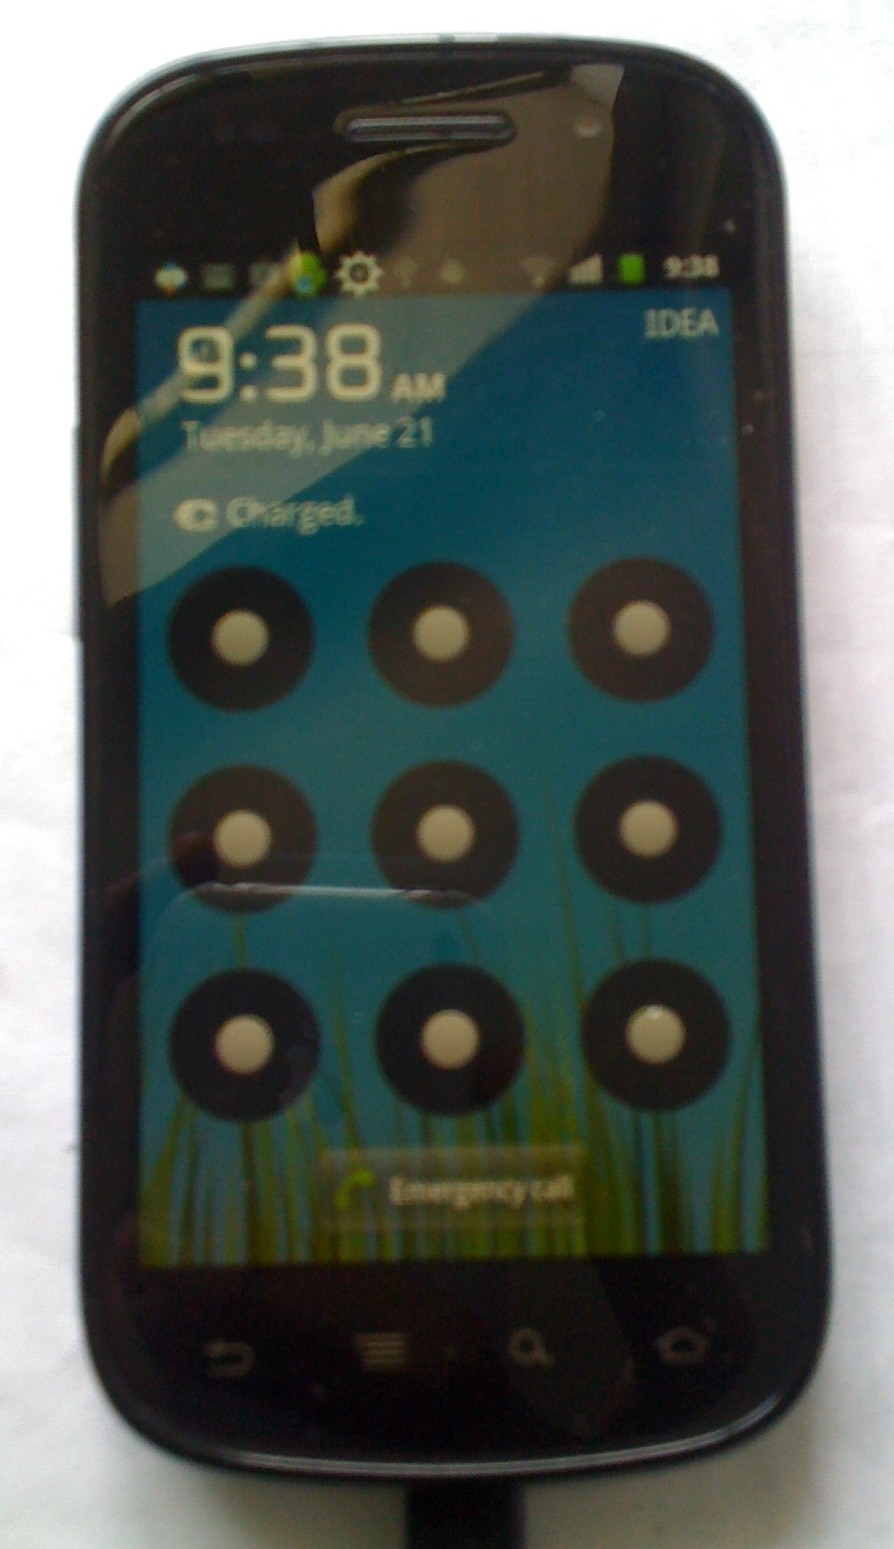
\includegraphics[height=3in]{figures/android_front}
    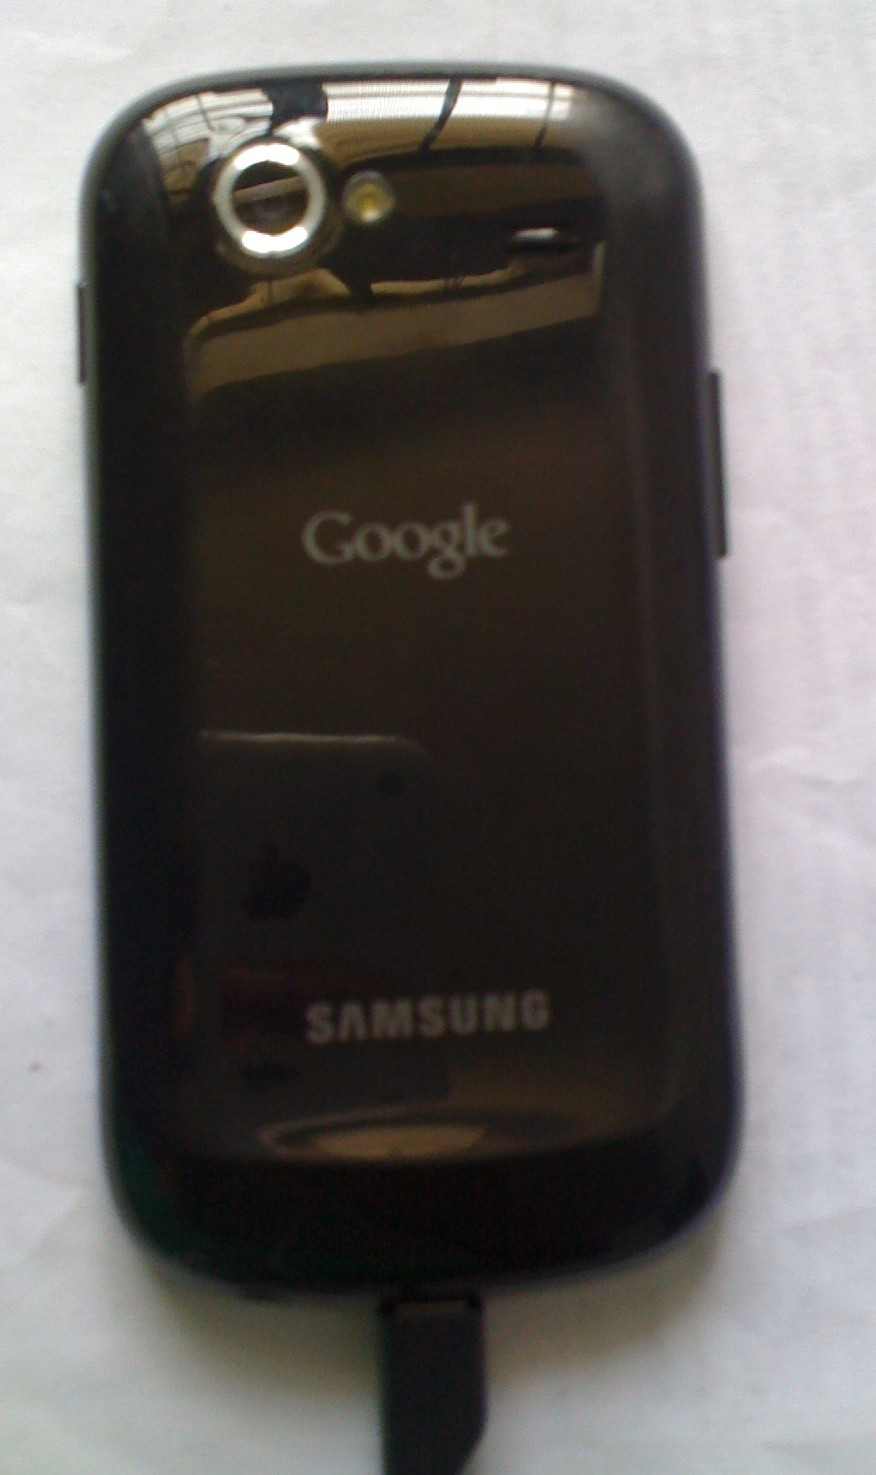
\includegraphics[height=3in]{figures/android_back}
\caption{Google Nexus S manufactured by Samsung}
\end{figure}



\section{Accelerometer}

The MEMS accelerometer on the Nexus S was subject to simple tests to determine 
its noise floor and the degree of separation between signal and noise.
Figure \ref{fig:accel_static} shows a plot of the accelerometer's raw output 
along the Z axis for a stationary device kept on a table. 

The noise level for the accelerometer was determined to be always less
than $0.6 m/s^2$. The acceleration peaks corresponding to regular walk steps 
usually lie around $2.0 m/s^2$. To allow for a reasonable noise margin and provide
sufficient cushion for additional noise introduced due to the dynamic nature of
walking, we choose a threshold of $1.3 m/s^2$ which is the mean value of the two
peak values. If the absolute value of the Z-axis acceleration sample is less
than this threshold, then the sample will be clamped to zero. For a smartphone
with a similar accelerometer sensor but with different noise characteristics,
the values of the threshold can be varied accordingly. 


\begin{figure}\centering
    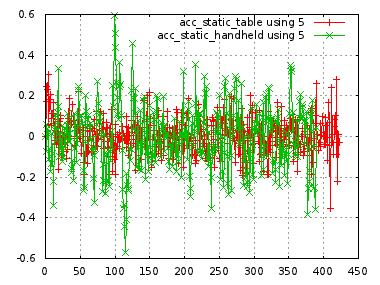
\includegraphics{figures/accel_static.png}
    \caption{Accelerometer Z axis readings when device stationary\label{fig:accel_static}}
\end{figure}

\section{Magnetometer}

The Nexus S comes with a built in MEMS magnetometer.
It measures the local magnetic field strength in $\mu T$.

In practical tests, the performance is reasonable but the magnetometer has a 
lot of sensor noise and suffers from sensor bias. For example, rotation of 
the smartphone through large angles introduces bias in the readings from the 
magnetometer. Similary, the magnetometer shows a small offset when the device is 
turned through 360 degrees.

Figures \ref{fig:angle_stationary_table} and \ref{fig:angle_handheld_standing}
show the behaviour of sensor readings under the 2 circumstances when the 
device is on a table and when it is held in the palm of the hand of a user.

\begin{figure}\centering
    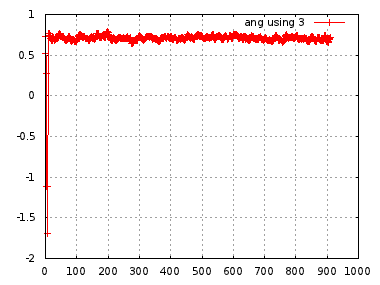
\includegraphics{figures/angle_stationary_table.png}
    \caption{Derived azimuth angle when smartphone on table\label{fig:angle_stationary_table}}
\end{figure}

\begin{figure}\centering
    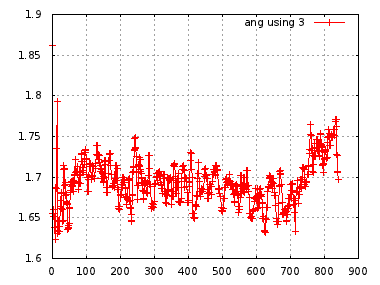
\includegraphics{figures/angle_handheld_standing.png}
    \caption{Derived azimuth angle when smartphone is held in the hand\label{fig:angle_handheld_standing}}
\end{figure}


\todo[inline]{Insert values for Standard deviation here}

These values are required to determine choice of parameters for the particle
filter that will be introduced later.

\subsection{Bias study}

Performing rotations in a slow and steady manner yields good results with little
or no bias and sensor lag. See figure \ref{fig:angle_180_rotation_table} which 
shows how the angle measurements behave when the rotated slowly and steadily.

There is only a slight sensor lag and bias visible. However, at steady state,
there is sensor noise of approximately 5 degrees present.

\begin{figure}\centering
    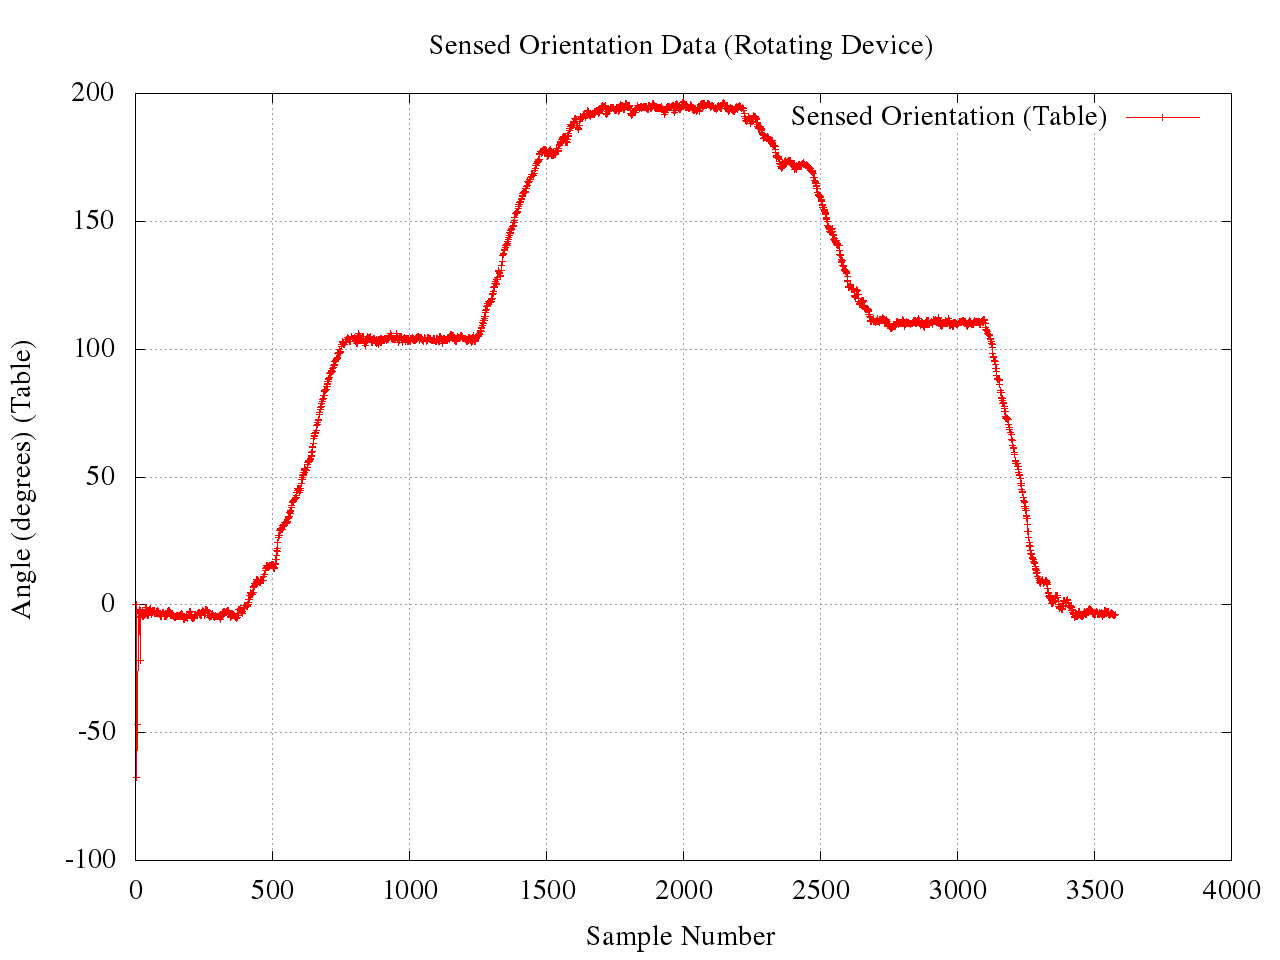
\includegraphics{figures/angle_180_rotation_table.png}
    \caption{Rotation of the phone through 180 degrees with pauses at 90 degrees.\label{fig:angle_180_rotation_table}}
\end{figure}


\subsection{Effect of motion}

Although the sensor measurements are stable when the device is on a table,
the measurements go haywire when the device is in a human's hand. See figure
\ref{fig:angle_180_corridoor} - a human is walking along a corridoor and he walks
back. The angle measurements of the return trip are offset by 180 degrees and
the two sets of measurements are compared. You can easily see a large variation
in the angles due to the motion of the human and the dynamic nature of the environment.
Sensor lag and long term sensor value drift is evident in the graph.
This dynamic variation of the measurement of the angle from magnetic north 
introduces error in the inertial navigation system.

\begin{figure}\centering
    \includegraphics{figures/angle_180_corridoor.png}
    \caption{Angle measurements when moving in opp directions.\label{fig:angle_180_corridoor}}
\end{figure}



\section{Wifi Signal Strength study}

The behaviour of the wifi signal strength distribution for a stationary laptop 
and smartphone was analyzed to characterize the input wifi signal.

\subsection{Short term duration}

Figure \ref{fig:closestAPshortterm} shows the variation of signal strength of 
the closest AP for a smartphone placed within a room in a NON-LOS configuration.

\begin{figure}\centering
    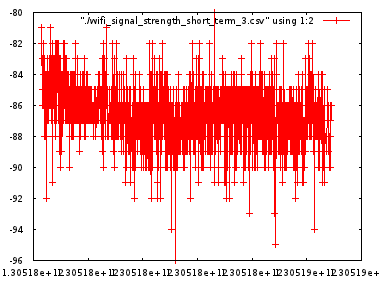
\includegraphics{figures/short_term_wifi.png}
    \caption{Variation of RSSI for closest AP. \label{fig:closestAPshortterm}}
\end{figure}


\subsection{During a thunderstorm}

Figure \ref{fig:closestAPthunderstorm} shows the variation of signal strength of
the closest AP for a smartphone placed in a room in NON-LOS configuration.

\begin{figure}\centering
    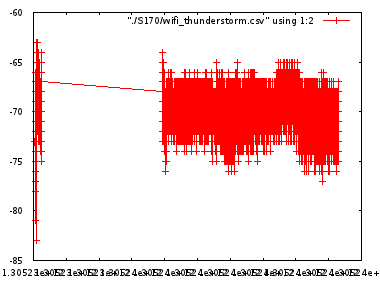
\includegraphics{figures/wifi_thunderstorm.png}
    \caption{Variation of RSSI for closest AP during a thunderstorm. \label{fig:closestAPthunderstorm}}
\end{figure}

\subsection{7 day study}

The Wifi AP RSSI values were monitored over a 7 day period (Jan 5 2011 - Jan 13 2011) from room S-152
and the resulting signal strength data was analyzed.

\begin{figure}\centering
    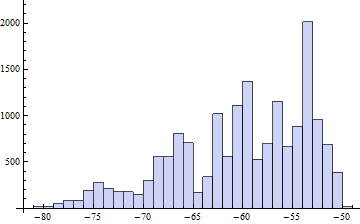
\includegraphics{figures/histogram_00_1C_F0_CB_EC_92.png}
    \caption{Distribution of RSSI values for the closest AP (00:1C:F0:CB:EC:92) \label{fig:histogram_00_1C_F0_CB_EC_92}}
\end{figure}

As you can see in Figure \ref{fig:histogram_00_1C_F0_CB_EC_92}, the signal strength
distribution is highly non-gaussian. This kind of distribution makes Kalman filters
unsuitable for use as the assumptions of gaussian (linear) distribution of 
input variables is unsatisfied.

\begin{figure}\centering
    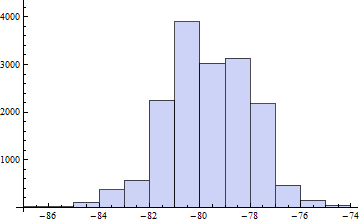
\includegraphics{figures/histogram_00_1C_F0_CB_EC_95.png}
    \caption{Distribution of RSSI values for the AP near S-170 (00:1C:F0:CB:EC:95) \label{fig:histogram_00_1C_F0_CB_EC_95}}
\end{figure}

\begin{figure}\centering
    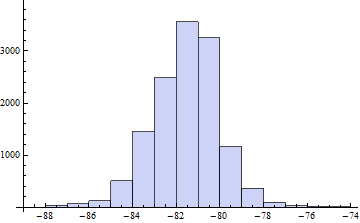
\includegraphics{figures/histogram_00_19_5B_77_A5_EE.png}
    \caption{Distribution of RSSI values for the AP near S-159 (00:19:5B:77:A5:EE) \label{fig:histogram_00_19_5B_77_A5_EE}}
\end{figure}

\begin{figure}\centering
    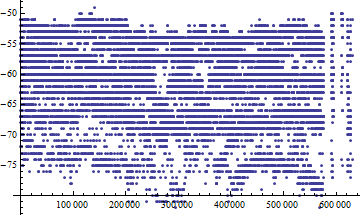
\includegraphics{figures/listplot_00_1C_F0_CB_EC_92.png}
    \caption{Point plot of RSSI values for the closest AP (00:1C:F0:CB:EC:92) \label{fig:listplot_00_1C_F0_CB_EC_92}}    
\end{figure}

\begin{figure}\centering
    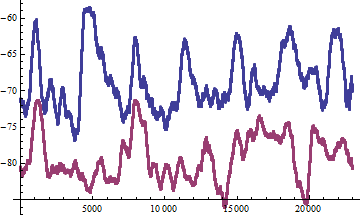
\includegraphics{figures/moving_average.png}
    \caption{3 hour moving average of RSSI values}
\end{figure}

Figure \ref{fig:histogram_00_19_5B_77_A5_EE} doesn't show such a pronounced non-gaussian
nature whereas Figure \ref{fig:histogram_00_1C_F0_CB_EC_95} shows more leanings towards a
non-gaussian distribution.

Figure \ref{fig:listplot_00_1C_F0_CB_EC_92} is the time domain plot of the signal strength
samples. As you can see, the samples can be spread over a large domain even if the 
sample times differ by a couple of hours. Thus we can safely conclude that the 
input wifi signal is a highly noisy source of information.

\section{Effect of motion on signal strengths}

To analyze the effect of motion on the RSSI values from the APs, a simple walking
test was done along a corridoor. The variation of RSSI values seen from the APs in
the corridoor are shown in \ref{fig:wifi_corridoor_walk}.

\begin{figure}\centering
    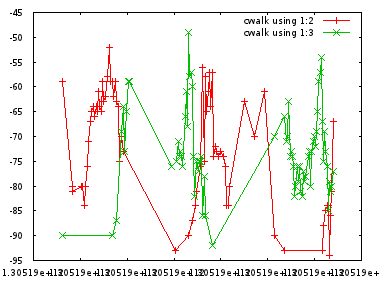
\includegraphics{figures/wifi_corridoor_walk.png}
    \caption{RSSI values for APs during a corridoor walk \label{fig:wifi_corridoor_walk}}
\end{figure}

\todo{Improve figure with more APs and path description.}

\subsection{Inferences}
Effect of orientation with respect to AP is important. Signal strength values
even in LOS situations don't always behave nicely.

\section{Wifi Surveying}

A $1m \times 1m$ grid was set up on the ground and wifi readings were taken at 8
different orientations per point on the floor.

\todo{Describe the setup better.}

\begin{figure}
    \centering
    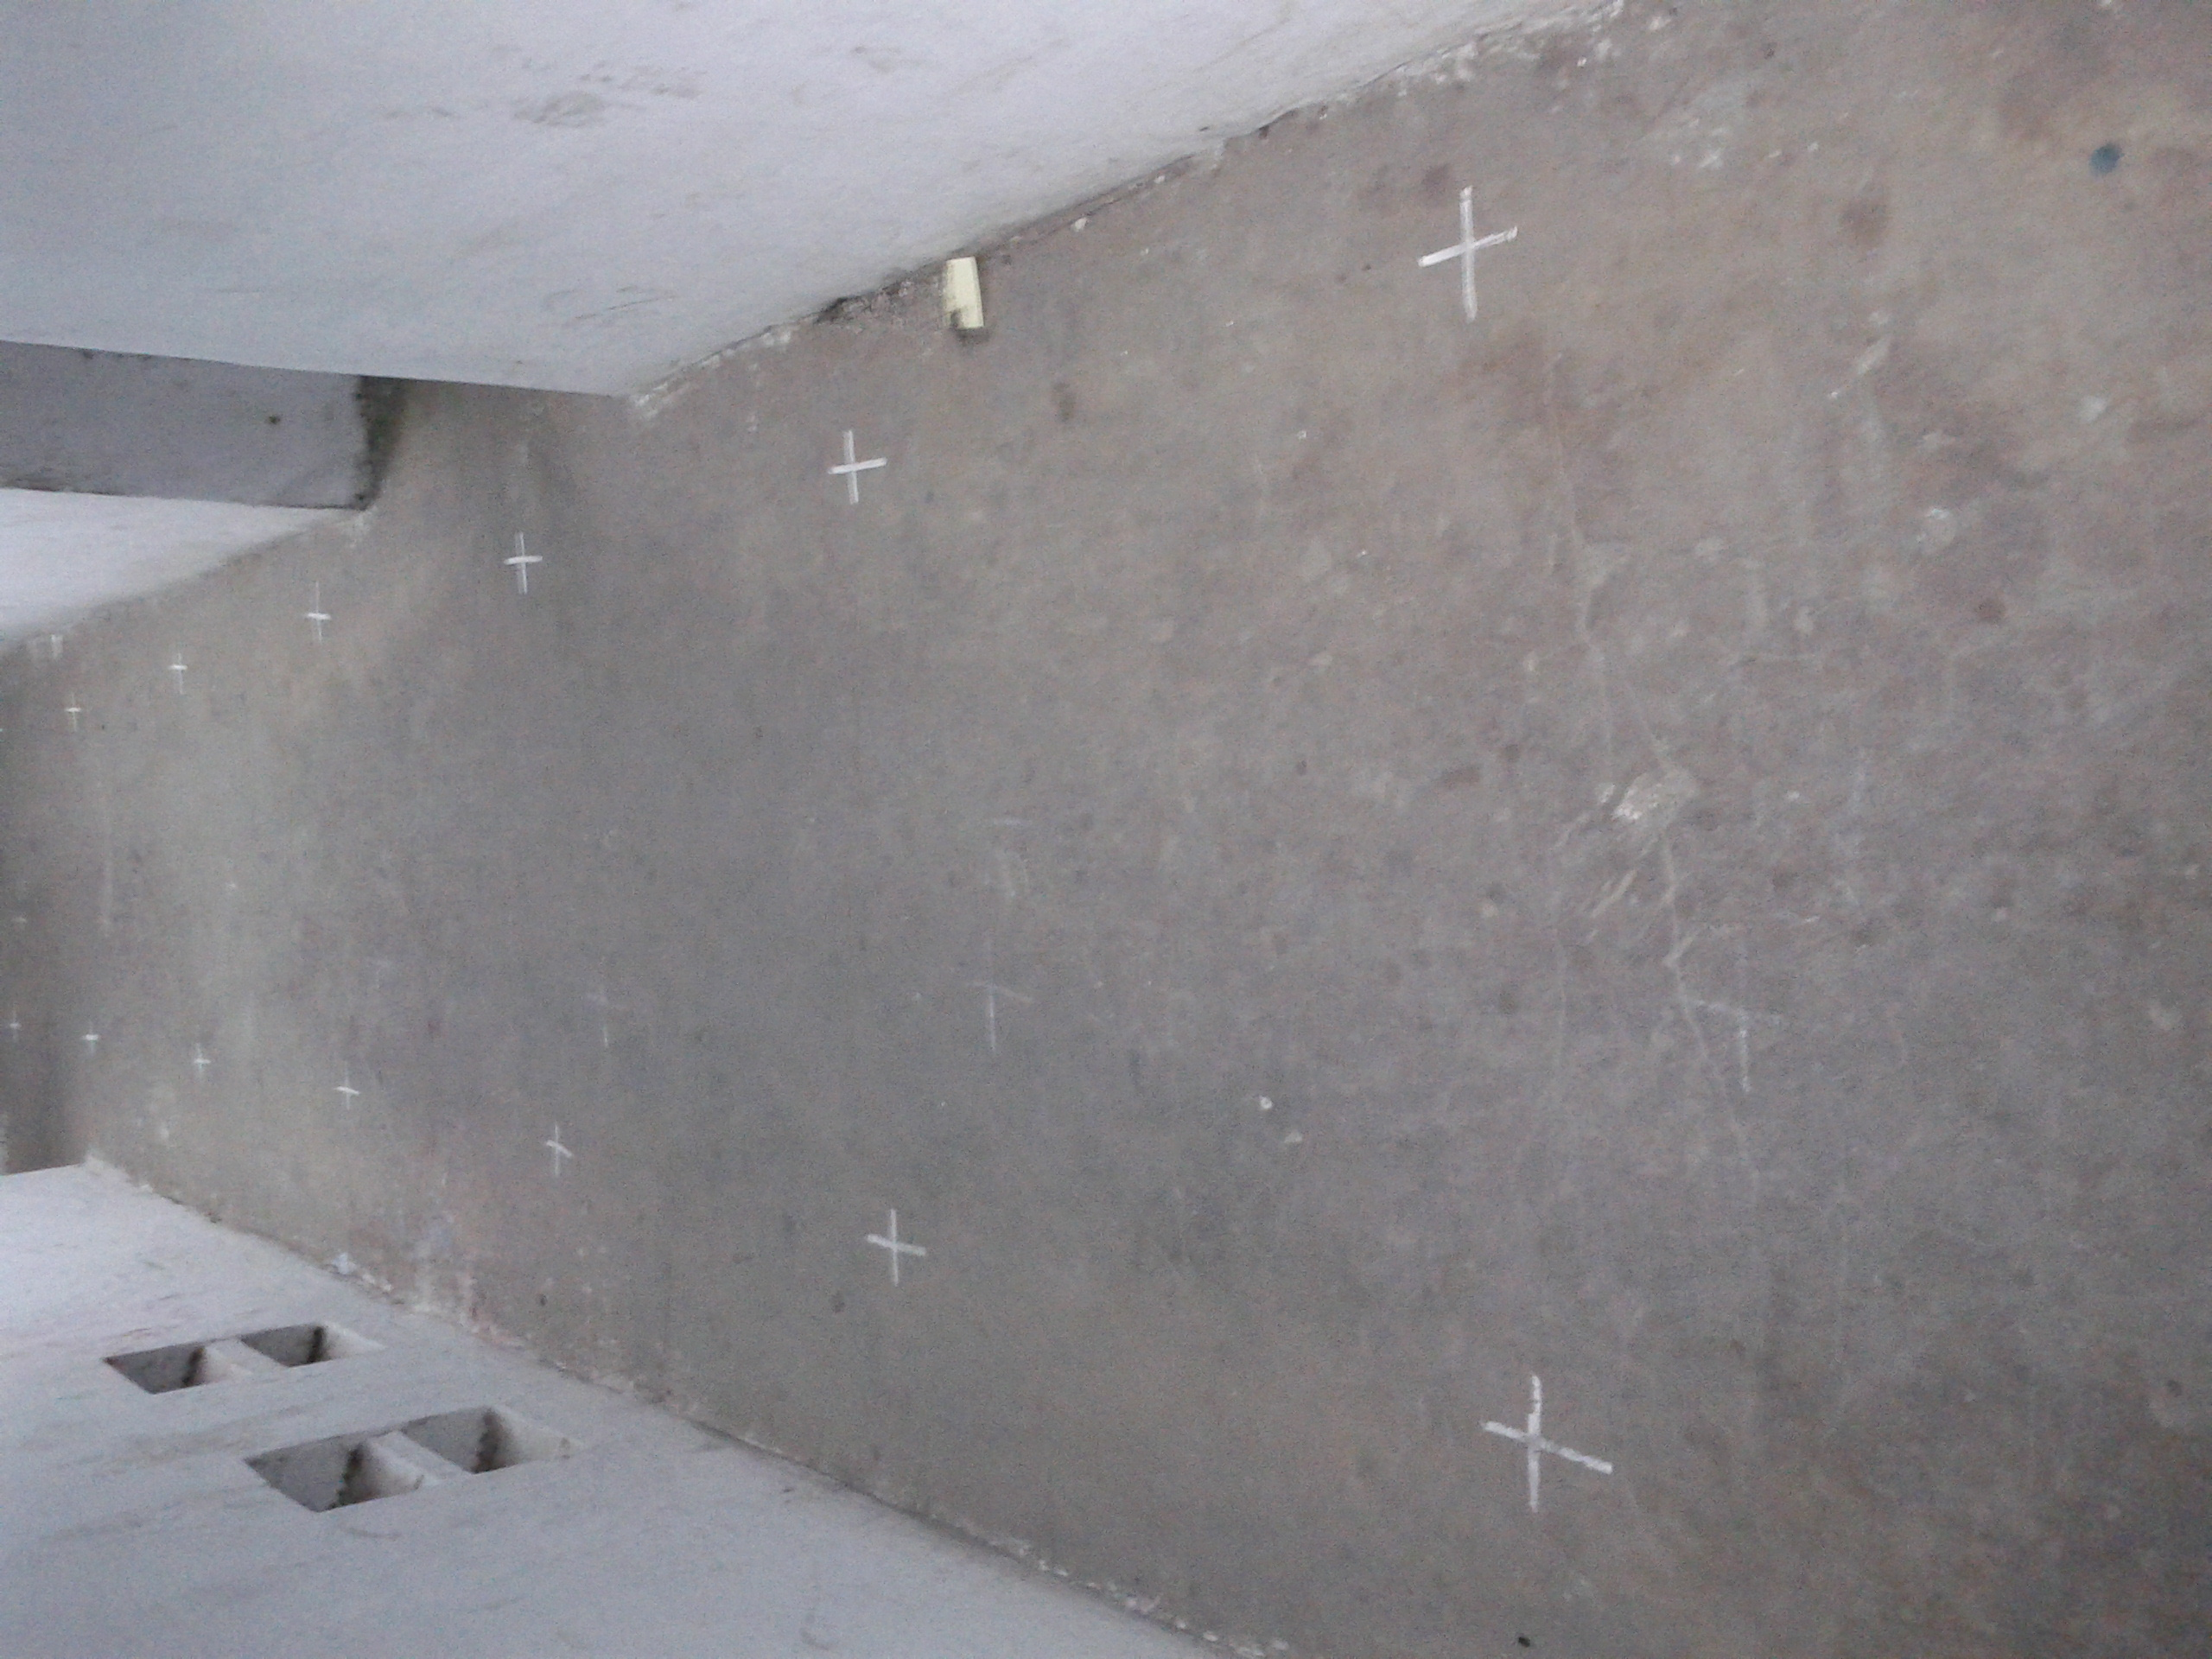
\includegraphics[width=5in,angle=270]{figures/grid_pic}
    \caption{Picture of the $1m \times 1m$ grid drawn on the floor}
\end{figure}

\section{Implementation of a KNN based positioning solution for KNN accuracy\label{sec:knn_pos}}

A KNN based location system was implemented to test location accuracy. 
This was work done as part of the project. Results are included here.

\begin{table}[h]
    \centering
    \caption{Performance of KNN based indoor positioning system \label{tab:knnperf}}
    \begin{tabular}{|l|c|c|c|}
    \hline
              & Mean Error $\bar{e}$ (m) & $\sigma_{error}$ (m) & $\bar{e} + 2 \sigma_{error}$ \\
    \hline
    \hline
    $K = 1$    & 2.8 & 2.7 & 8.2 \\
    $K = 2$    & 2.8 & 2.7 & 8.2 \\
    $K = 3$    & 2.7 & 2.7 & 8.1 \\
    $K = 4$    & 2.3 & 2.8 & 7.9 \\
    \hline
    \end{tabular}

\end{table}


\subsection{Improvements}
Use of SVM is likely to improve the accuracy further at room level. [Redpin]


\section{Dead Reckoning by direct integration: What doesn't work}
\section{What Doesn't work}
\todo{Fix this!}
Acceleration of the human body is too slow compared to gravity. Simple orientation changes produce high changes in acceleration along axes which are very difficult to filter out.
Numerical integration generates errors too quickly. With a high sampling rate, errors balloon.
Using the gyroscope for step detection (similar to foot mounted devices [insert reference]) – doesn’t work.


\section{Other issues}
Sensor noise, instability and bias. Effect of gravity and orientation on readings. Weather.

